\documentclass[fontsize=11pt]{article}
\usepackage{amsmath}
\usepackage{hanging}
\usepackage{setspace}
\usepackage{graphicx}
\usepackage[hidelinks]{hyperref}
\usepackage[utf8]{inputenc}
\usepackage[margin=0.75in]{geometry}

\title{Misinformation Represented in Tweets Throughout the COVID-19 Pandemic}
\author{Muhan (Elsie) Zhu, Ron Varshavsky}
\date{Tuesday, December 14, 2021}

\begin{document}
    \maketitle

    \section*{Problem Description and Research Question}

    Throughout the COVID-19 Pandemic, there has been an influx of rumours and misinformation related to the virus and how different countries responded. The World Health Organization has dubbed this an ``Infodemic” alongside the current worldwide pandemic. This widespread misinformation has been catastrophic in many areas. A prime example is the “cure” for COVID-19 which circulated near the beginning of the pandemic. This ``cure” involved injecting bleach into your arms (van der Linden et al., 2020). Such rumours are not only false, but they are dangerous. In fact, this false fact was so widespread that the reported cases of accidental poisoning due to bleach in Americans doubled in March and April of 2020 (Bowden, 2020). The effects of a singular rumour were so detrimental that it compromised the lives of many people; such widespread misinformation is quite literally deadly. Such misinformation has changed over time, however it has never been fully eradicated from word of mouth, such as the rumour that taking a potentially dangerous dose of Ivermectin could reduce COVID-19 symptoms (U.S. Food and Drug Administration, 2021). This rumour, like the previous one mentioned, can put numerous lives at risk. We researched how public conversation surrounding the virus and misinformation have been impacted over time during the pandemic, and if these time frames coincided with any major milestones within the pandemic (i.e lockdown, vaccine distribution). We found evidence relating to the periods of time within the pandemic when influxes of misinformation took place. This allowed us to hypothesize the mistakes that we, as a society, made during the course of the pandemic which caused this spread of false, dangerous information. In order to quantify our research, we asked the question: \textbf{In what way, quantitatively, has misinformation in discourse on Twitter surrounding the COVID-19 pandemic changed over the course of the pandemic?}

    \section*{Dataset Descriptions}

    The source for our myths is the Newsguard Covid Myths website. Here, we simply scraped each myth from their site, and removed the characters ``MYTH: " from the beginning of each scraped line. The NewsGuard website can be found here: \href{https://www.newsguardtech.com/special-reports/coronavirus-misinformation-tracking-center/}{https://www.newsguardtech.com/special-reports/coronavirus-misinformation-tracking-center/}. \\
    Another source we used for our myths was creating a separate file where we would input known misinformation that was skipped over in the NewsGuard website because they were removed as the site updated. We then combined both this source and the previous source into one file for a single dataset of ``COVID-19 myths", which we used to detect misinformation.\\
    To find the tweets relating to COVID-19, we used the dataset ``COVID-19 Twitter Dataset with Latent Topics, Sentiments and Emotions Attributes". It can be found here: \href{https://www.openicpsr.org/openicpsr/project/120321/version/V11/view;jsessionid=EB090760F70409E47B82FC0137D7B1A1}{https://www.openicpsr.org/openicpsr/project/120321/\\version/V11/view;jsessionid=EB090760F70409E47B82FC0137D7B1A1}. This csv dataset contains 198 million Twitter tweet ID's, but does not contain the tweets themselves. Evidently, this would be very time consuming to compute on, so we took a smaller sample size by only using 1 in 30 000 lines of the dataset, resulting in about 6600 tweet id's to compute on. From here, we had to collect our own tweet dataset, as the dataset provided only contains tweet ID's, due to Twitter's API policy. As such, we used the Twitter API to get the text of each tweet by its ID. We then gathered each of these tweets into a separate file and used this as a dataset to compute on.\\
    Finally, we compiled a list of common negation words from Grammarly into a text file, to use for the false-positive portion of our misinformation detection algorithm. The data we scraped can be found here:\\ \href{https://www.grammarly.com/blog/negatives/}{https://www.grammarly.com/blog/negatives/}.

    \section*{Computational Overview}

    \textbf{Data Filtering}\\
    After downloading the Twitter dataset, we immediately isolated just the ID's from the dataset, as it contained other information not relevant to our project. We did this in \texttt{pull\_tweets.py} inside the function \texttt{isolate\_ids()}. Here, it opens the full dataset csv file, and then splits the csv by its commas and writes the \texttt{twitter id} columns into a new file generated called \texttt{twitter\_ids} with no file extension, in the directory \texttt{./data/twitter\_ids}. From here, we used \texttt{pull\_direct\_tweets()} in the same file to use the IDs we isolated to request the Twitter API and actually get a response containing the text of the tweet. Unfortunately, due to the structure of Twitter's API, there is a rate limit of 900 requests per 15 minutes, so we had to run this function multiple times, storing data in multiple files, and then combining it in the next function we used, \texttt{compile\_into\_file()}, which took all of the files we first generated, and wrote them into a single file named \texttt{filtered\_twitter\_ids\_compiled}, with no file extension, stored in the directory \texttt{./data/filtered\_twitter\_ids\_compiled}. From here, we ran \texttt{sort\_by\_month} to sort the compiled file into multiple files separated by the month and year that each tweet was posted. This function accomplished this by creating a list of open files for each month/year combination in the dataset, and then reading through each line of the compiled Twitter API responses, and then running a helper function \texttt{isolate\_text\_write\_to\_file}, which isolated the text, and based on what year and month combination the Tweet was posted, wrote the tweet text into that file. After all of this was completed, we successfully had thousands of tweets each sorted into a file based on the month and year they were written, waiting to be computed on. \\
    \hfill\break
    \textbf{Data Computing} \\
    Once the data was filtered, the data was computed on. This was done in the file \texttt{compute\_similarity.py}. In this module, a function named \texttt{output\_myths\_count\_into\_file} is called, with a filename as its parameters. This filename is a file of combined myths that were assembled through web-scraping. Essentially, this file calls a helper function and then writes the returned value from the helper function into a file. The helper function is named \texttt{get\_myths\_for\_every\_month}, and it computes the misinformation counts that were generated for every month available in the dataset. It does this by going through every month and year combination, and then running another helper function, then appending the returned value to a list. This helper function is titled \texttt{compute\_misinformation\_month}, and it returns the number of misinformation detected for the inputted month as well as the rate of misinformation. Essentially, using a list of myths, this function checks every line of the dataset for the month it was inputted through the misinformation detection algorithm, and then writes it to a file. To determine if a string is misinformation, it runs the \texttt{is\_misinformation} function from the \texttt{similarity} module which we wrote. To determine if a string is misinformation, the function first runs \texttt{check\_similarity\_score}. This function uses \texttt{FuzzyWuzzy}'s \texttt{token\_sort\_ratio()} function, which returns a score from $0 - 100$ on how similar two strings are. By setting a threshold at $70\%$, it is able to identify when a string mostly contains a myth, although some are missed. The second part of the \texttt{is\_misinformation} function is a second function called \texttt{is\_false\_positive}, which uses a list of negation words to determine if a sentence is actually NEGATING a myth, thus would not be misinformation. This function simply checks if there is a negation word, and returns True if there is. Putting both of these together, \texttt{is\_misinformation} returns True if a function both has a similarity score above the threshold, and is not a false positive. Otherwise, the function returns False. \\
    \hfill\break
    \textbf{Data Visualization}\\
    In order to visualize this data, we settled on using the Pygame library. Specifically, in $\texttt{visualize\_data.py}$, the \texttt{visualize()} function does most of the work. The function draws 3 rows of buttons, with 7 buttons per row, accounting for every month of the dataset. The function also has an empty gray bar which can be likened to a ``progress bar". By checking the mouse position on mouse clicks, we can turn the buttons functional. Simply, when a specific part of the screen is pressed, which is tied to a certain month/year combination, the progress bar will smoothly fill to a certain percentage for that month. This was chosen to be the way to visualize the data, because it allows for all of the data to be seen easily, and it is interactive. It gives the user more control over which data they want to see, as they are the ones who select which month/year combination to open.

%First, we will need to filter the dataset to only contain verified false rumours. Since the dataset is only updated to April 31, 2020, we will also likely need to web-scrape more COVID-19 misinformation from other verified sources such as NewsGuard, or Snopes. To perform this web-scraping, we will use the scrapy library. With the web-scraped data, we will then clean up this data by removing unnecessary words accidentally picked up by the scraper. For example, NewsGuard has a list of COVID-19 myths, but each point begins with "MYTH:". Our cleaning algorithm would remove this first word. We will then append this cleaned up web-scraped data to the previous dataset. From there, we will use this filtered dataset by cross-referencing the articles with each verified false rumour using fuzzy string matching. Fuzzy string matching is a method of checking how close two strings are using Levenshtein distance. This type of string comparison is vital for this type of computation because the articles will typically not match exactly what the rumour string is, but will contain similar keywords. To perform this fuzzy string matching, we will use the ``Fuzzy Wuzzy" library available on PyPi, which contains a function titled ``Partial Token Sort", which returns a similarity score of two strings regardless of the order of the words. With this model of analysis, we will run this algorithm on top articles from each month of the pandemic since December 2019 to determine how many articles contain misinformation, as well as what kind of misinformation they contain. With the evidence gathered, we will then be able to see as well as visualize the change in the amount of misinformation detected in top articles over time as a graph. We plan to add an interactive element as well, perhaps to click on the graph and see a breakdown of what kinds of misinformation were most common for the month.

    \newpage
    \section*{Results}
    On our computations on the data, we found the following results:\\

    \begin{tabular}{|c|c|c|}
        \hline
        \textbf{Month/Year} & \textbf{\% Tweets w/ Misinformation} & \textbf{Hard Values Tweets w/ Misinformation} \\
        \hline
        Jan 2020            & 4.8\%                                & 20                                            \\
        Feb 2020            & 19.5\%                               & 143                                           \\
        Mar 2020            & 28.5\%                               & 154                                           \\
        Apr 2020            & 24.9\%                               & 173                                           \\
        May 2020            & 10.2\%                               & 37                                            \\
        Jun 2020            & 18.9\%                               & 88                                            \\
        Jul 2020            & 26.2\%                               & 95                                            \\
        Aug 2020            & 5.7\%                                & 22                                            \\
        Sep 2020            & 10.8\%                               & 27                                            \\
        Oct 2020            & 10.9\%                               & 56                                            \\
        Nov 2020            & 36.6\%                               & 134                                           \\
        Dec 2020            & 8.8\%                                & 34                                            \\
        Jan 2021            & 27.0\%                               & 97                                            \\
        Feb 2021            & 6.5\%                                & 18                                            \\
        Mar 2021            & 34.6\%                               & 79                                            \\
        Apr 2021            & 13.9\%                               & 50                                            \\
        May 2021            & 8.6\%                                & 23                                            \\
        Jun 2021            & 6.0\%                                & 12                                            \\
        Jul 2021            & 5.8\%                                & 16                                            \\
        Aug 2021            & 23.8\%                               & 70                                            \\
        Sep 2021            & 0.0\%                                & 0                                             \\
        \hline
    \end{tabular}


    \section*{Instructions to Reproduce}

    \begin{flushleft}

        \textbf{Obtaining Datasets:}\\

        Step 1: Download the necessary files from \textbf{UTSend}:\\
        \textbf{Claim ID}: sqiomTmz6ukdcSCc \\
        \textbf{Claim Passcode}: cUpxkZGZusgCCmJT
        \hfill\break

        \textbf{Note, UTSend will download the pre-processed version of this tweets dataset. Unfortunately, due to the Twitter API's rate limiting, it is difficult to reproduce gathering tweet texts from their IDs.}\\

        Once you have downloaded the necessary data, as well as downloaded the Python files from MarkUs, your directory should look as follows:

        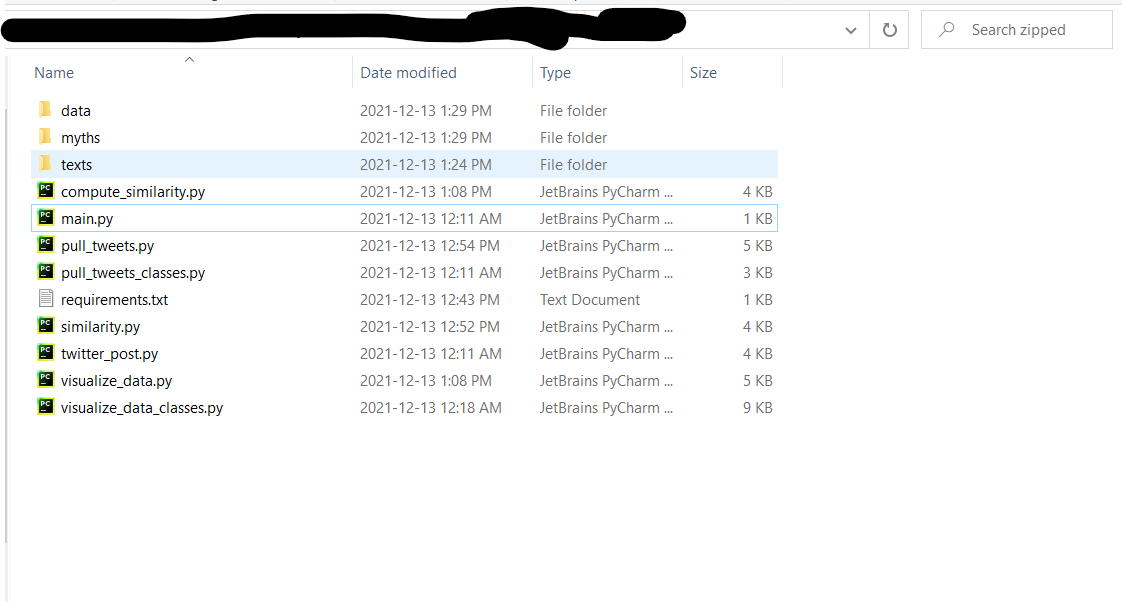
\includegraphics[scale=0.5]{LATEX_directory_after_download.png}

        \textbf{Please note, when you unzip the file downloaded from UTSend, it will extract into a new folder. We do not want this. Instead, cut all the folders inside of the extracted folder and move them into the same folder as all of the Python files.}
        \\

        In the main directory, there are
        \texttt{filtered\_twitter\_ids\_compiled} is the main dataset of filtered Twitter IDs, generated using \texttt{twitter\_post.py}, \texttt{pull\_tweets\_classes.py}, and \texttt{pull\_tweets.py}.

        \texttt{twitter\_post.py} requests the server and gets tweet IDs to search on the API.

        \texttt{pull\_tweets\_classes.py} generates a list of needed month-year combinations.

        \texttt{pull\_tweets.py} randomly pulls valid tweets using their IDs from the Twitter dataset and writes them into \texttt{filtered\_twitter\_ids\_compiled}.
        \hfill\break

        \texttt{requirements.txt} is the required file that lists all the external libraries that we used.

        \texttt{extracted\_myths.txt} is the file that contains all of the myths that we extracted from the NewsGuard website using our NewsGuard Spider that will be used to compute misinformation.

        \texttt{extra\_added\_myths.txt} is the file that contains our added myths that were not listed on the website that will be used to compute misinformation.

        \texttt{negation\_words.txt} is the file that contains negated words that will be used to compute similarity.
        \hfill\break

        \texttt{compute\_similarity.py} computes the amount of misinformation is found in tweets from each month and outputs it into a file.

        \texttt{similarity.py} is a module that checks if two strings are similar - this is used by \texttt{compute\_similarity.py}.
        \hfill\break

        \texttt{visualize\_data\_classes.py} provides the necessary information to \texttt{visualize\_data.py} to create a row of buttons in Pygame.

        \texttt{visualize\_data.py} visualizes all of our data.
        \hfill\break

        \texttt{main.py} is the required main program file.
        \hfill\break

        Inside of each folder, there should be data, and inside of \texttt{myths}, there should also be a web-scraper named \texttt{newsguard\_spider.py}. Each folder should look as follows:

        \textbf{The data folder}:\\

        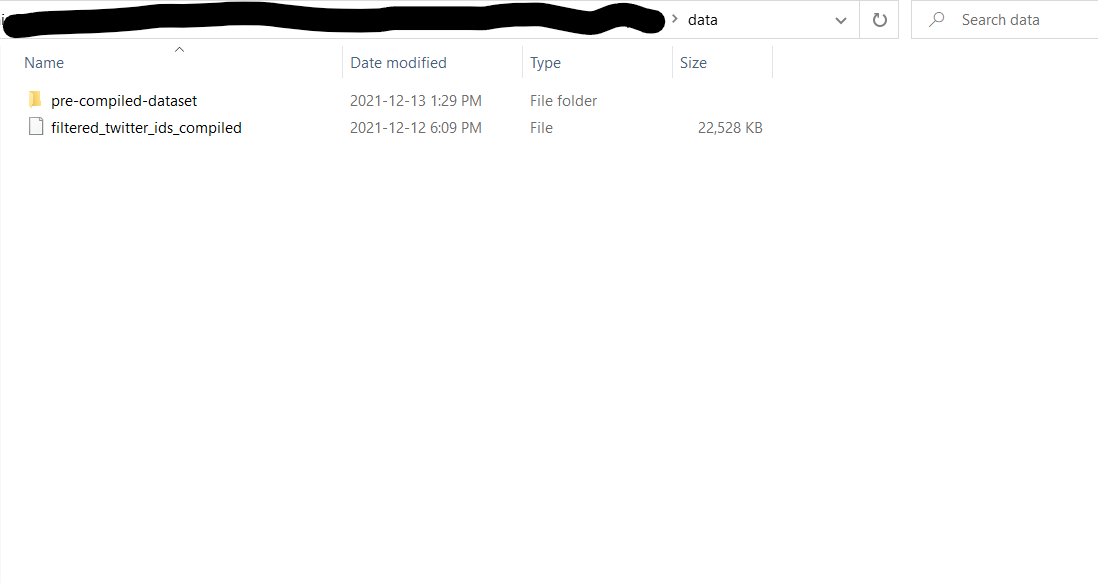
\includegraphics[scale=0.5]{LATEX_data_folder.png}\\
        \textbf{The myths folder}:\\
        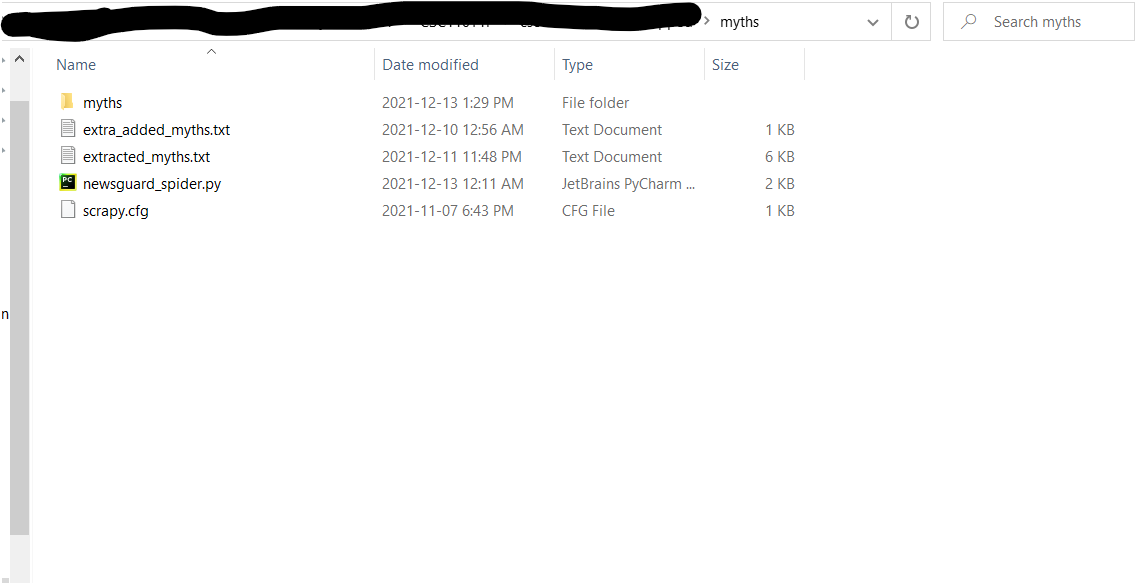
\includegraphics[scale=0.45]{LATEX_myths_folder.png}

        \newpage

        \textbf{The texts folder:}\\

        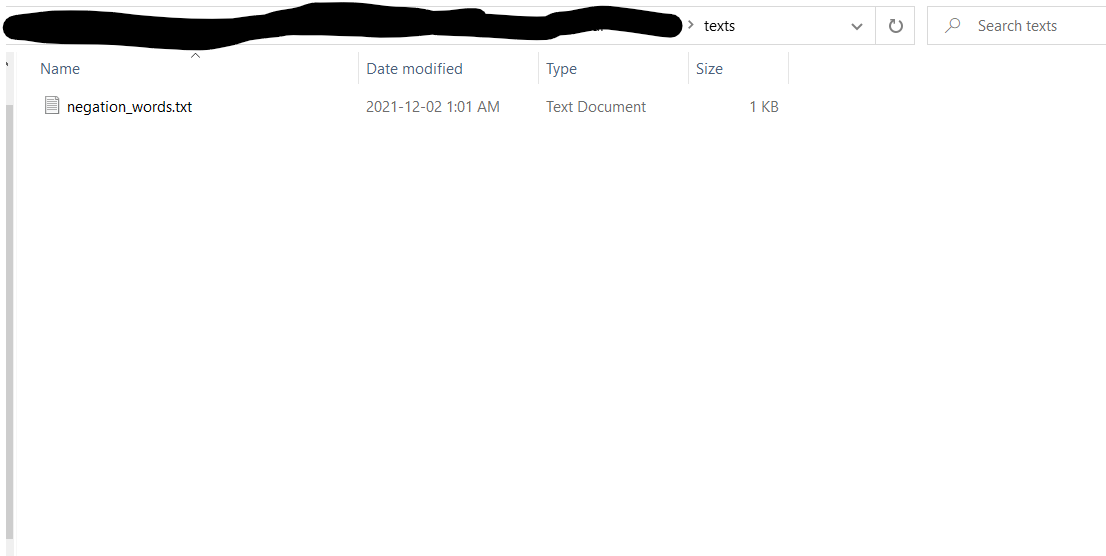
\includegraphics[scale=0.5]{LATEX_texts_folder.png}

        Notice that there is also a subfolder inside of \texttt{data} named \texttt{pre-compiled-dataset}. This folder is only necessary if the computations on the data are too time consuming to reproduce, and the grader wishes to test the visualization function. It should look as follows inside:

        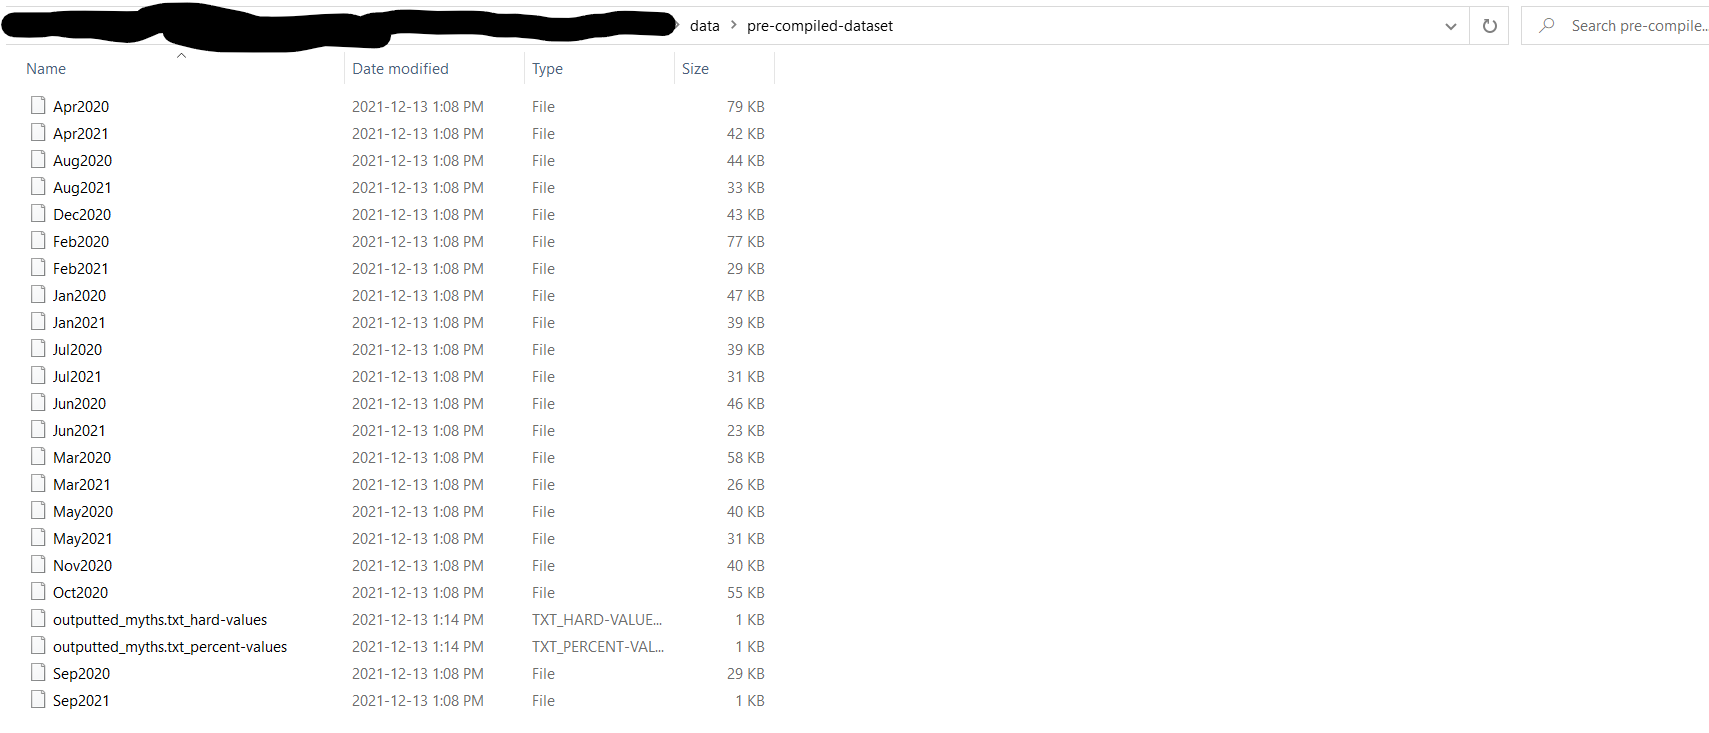
\includegraphics[scale=0.5]{LATEX_compiled_dataset.png}

        \textbf{!!!OPTIONAL!!! Refreshing the list of myths scraped from NewsGuard:}\\
        If you would like to refresh the myths scraped from the NewsGuard website, run \texttt{newsguard\_spider.py} and then go into the Command Line and change the directory to the project folder, in the \texttt{myths} subfolder. Relative to the main project folder, it should be in \texttt{./myths/}. Then, run the command \texttt{scrapy runspider newsguard\_spider.py} in the command line. This should update the \texttt{extracted\_myths.txt} file with an updated set of scraped myths from the NewsGuard website.
        \hfill\break

        \textbf{Running The Program:}

        Step 1: Open main.py and run it.
        \hfill\break

        Step 2: Wait for the hard values and percent values for misinformation in each month in our analysis to generate. This may take a long time depending on your computer's processing speed.
        \hfill\break

        NOTE: If Step 2 takes too long, we have provided a sample of data that we have already generated. You can use this instead of waiting for the program to generate a new set of values. To use this, please comment out line 20 in \texttt{main.py}, move every file in \texttt{./data/pre-compiled-dataset} up a folder into \texttt{./data}. Then, re-run \texttt{main.py}.
        \hfill\break
        \newpage
        Step 3: When the Pygame window opens up, you will see a few rows of buttons at the top of the page, labelled with the month and year; the percent value of the misinformation found for that month (this will be empty at first); and the bar representing this percentage (this will be empty until you select a month). Simply click on the desired month to see the rate of misinformation found in that month in percentage value, and the bar that visually represents this percentage value.
        \hfill\break

        On startup, the visualizer should look as follows:\\
        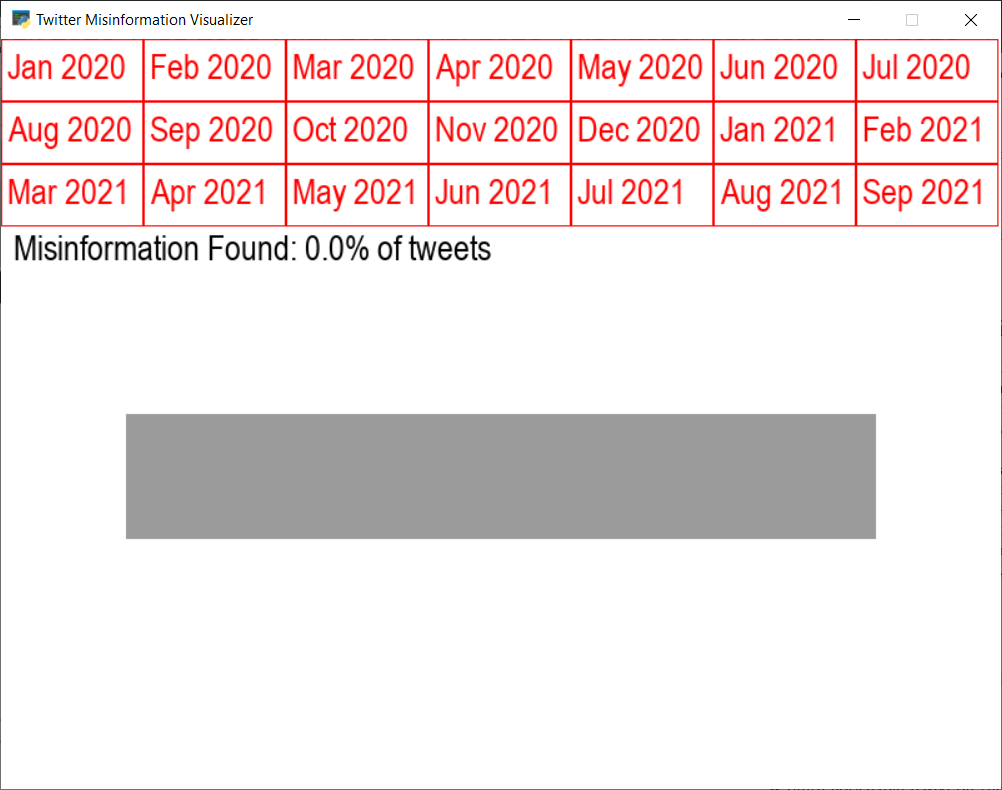
\includegraphics[scale=0.7]{LATEX_pygame_on_startup.png}\\
        If it does not look like the screenshot, there is a \textbf{glitch with \textit{PYGAME}}, and to fix it, you should \textbf{minimize, not close} the window and then reopen the window, and the glitch should be fixed.\\
        When you click on a month/year combination, said button should turn green, and the progress bar will slowly fill up with the percentage of misinformation it detected. It will look as follows:\\
        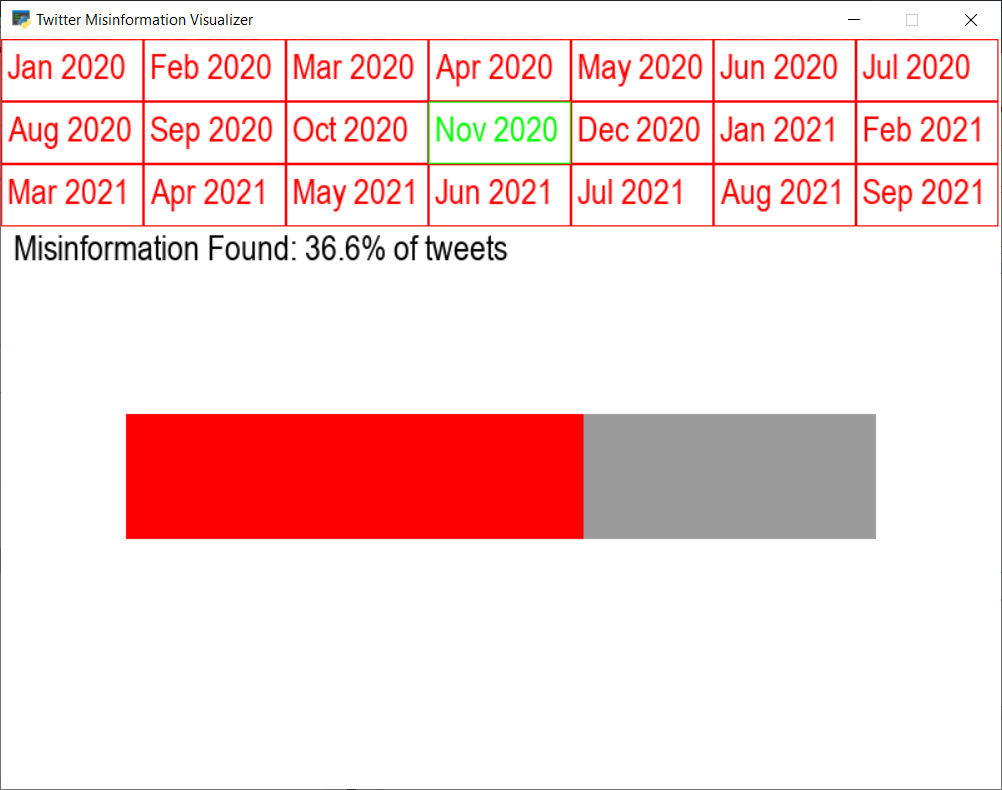
\includegraphics[scale=0.7]{LATEX_pygame_on_click.png}.


    \end{flushleft}


    \section*{Changes Between Proposal and Final Submission}
    Between the proposal and the final submission, we made a few changes. First, we did not include the original dataset of myths we outlined in the proposal. This was because the dataset only contained myths for about three months worth of the pandemic, which made it largely irrelevant. Due to the immense number of computations performed by our algorithm to check for misinformation, we concluded that the few extra myths would not outweigh the extra time it would take to compute on the tweet data. \\
    Another change we made was switching from searching for misinformation within news articles, to searching for misinformation within tweets on Twitter. We settled on this change because most news agencies perform intense fact checking for their articles, and if they do accidentally release misinformation, many will retract said articles making the entire project idea rather cumbersome, as there would be little misinformation found. On the other hand, we found that on Twitter, many people would simply post without fact checking, which allowed for widespread misinformation. Although Twitter does its due diligence to try to flag, and in some cases remove misinformation, they are bound to miss tweets, which was quite noticeable based on the results of our computations. We also came to the conclusion that discussions on Twitter have an immense impact on real world news, alongside the media. In fact, according to Pew Research, about 50\% of adults in the United States say they either sometimes, or often get their news from social media. As such, misinformation within social media plays a very big role in the world, and we decided it would be beneficial to research this.

    \newpage

    \section*{Discussion}
    \begin{flushleft}

        The results from our computations show a very interesting trend: real world news impacted misinformation. The months that yielded the highest rates of misinformation among tweets on Twitter were April 2020, November 2020, January 2021, March 2021, April 2021, May 2021, and August 2021. These highlighted months coincide with the dates where worldwide COVID-19 cases spiked or the month following those months, where many areas of the world went into lockdown as an attempt to lessen the spread of the virus. Similarly, on the months where COVID-19 vaccines first became widely available and encouraged by multiple countries' governments, such as January 2021, the rate of misinformation in tweets also spiked. Both lockdowns and vaccines pertaining to COVID-19 are considered `controversial' - they give rise to public disagreement and they tend to trigger strong opinions or emotions in many individuals. This may explain the spikes in rates of misinformation in Twitter. Moreover, the months where the lowest rates of misinformation were found on Twitter were August 2020, February 2021, June 2021, and July 2021. These months coincide with the points during the COVID-19 pandemic where worldwide cases were the lowest and when many regions of the world, as a result of these low number of cases, lifted or began to lift their lockdown restrictions. This data definitely helps answer the research question. Our data explicitly shows how misinformation within tweets on Twitter changed throughout the pandemic, and during which months spikes in misinformation rates occurred.\hfill\break

        There were a number of limitations encountered throughout the development of this project. Due to Twitter terms of service, the dataset we used for the tweets did not contain any text from the tweets, instead storing the ID linking to the tweet. This caused a limitation with how accurate our data can be, as some of the tweets we attempted to analyze were deleted. Another limitation is with the FuzzyWuzzy library. Unfortunately, calculating Levenshtein distance is rather time consuming with this library, so once all the Twitter data is generated and filtered, computing on said data to find misinformation can take upwards of 15 minutes for all 21 months. Finally, a limitation with the algorithm is the way misinformation itself was detected. Using fuzzy string matching unfortunately does not account for words that are in different tenses, or different variations of the same word. For instance, `consult' versus `consultation' or `consulting'. With our implementation of fuzzy string matching, only one of these three would be picked up by the algorithm. Another limitation involves synonyms. To illustrate, with words such as `sickness' and `illness', the algorithm would struggle detecting misinformation where the sample text does not match the inputted string. \hfill\break

        To further explore the topic of the Change in Misinformation in Tweets on Twitter, we can improve the misinformation algorithm so that it is faster or more accurate. At this moment, the misinformation algorithm that calculates the amount and rate of misinformation in tweets is relatively slow - fuzzy string matching is calculated several times. To improve this project, we can incorporate machine learning instead of using fuzzy string matching, which would improve the accuracy of the misinformation algorithm by matching words by their root meaning, instead of their exact composition. For example, the algorithm would have the ability to identify two words with the same root as having the same relative meaning, such as ``combine" and ``combination." The algorithm could also be improved so that it could recognize two words that are synonyms as having the same meaning, such as `sick' and `ill.' Additionally, to further explore this topic, we can analyze the main topics that contribute the most to each month's rate of misinformation - for example, we can calculate the rate of each trigger word for misinformation: whether that be ``lockdown", ``vaccine", etc.

    \end{flushleft}

    \newpage

    \section*{References}

    \begin{doublespace}
        \begin{hangparas}{0.25in}{1}
            Bowden, J. (2020, May 12). Accidental poisonings from bleach and other disinfectants spiked amid coronavirus. TheHill. Retrieved November 4, 2021, from https://thehill.com/policy/healthcare/497312-accidental-poisonings-from-bleach-and-othr-disinfectants-spiked-amid.

            Bryner, J. (2020, April 24). Disinfectant injections are a really bad idea. LiveScience. Retrieved November 4, 2021, from https://www.livescience.com/disinfectant-injections-coronavirus-dangerous.html.

            Edward, A. (2021, June 13). An Extensive Guide to collecting tweets from Twitter API v2 for academic research using Python 3. Retrieved December 12, 2021, from https://towardsdatascience.com/an-extensive-guide-to-collecting-tweets-from-twitter-api-v2-for-academic-research-using-python-3-518fcb71df2a

            Gupta, Raj, Vishwanath, Ajay, and Yang, Yinping. (2021). COVID-19 Twitter Dataset with Latent Topics, Sentiments and Emotions Attributes [Data set]. https://www.openicpsr.org/openicpsr/project/120321/version/V11/\\view;jsessionid=EB090760F70409E47B82FC0137D7B1A1

            NewsGuard. (2021, November 1). Coronavirus Misinformation Tracking Center. NewsGuard. Retrieved November 4, 2021, from https://www.newsguardtech.com/special-reports/coronavirus-misinformation-tracking-center/.

            Office of the Commissioner. (2021, September 7). Why you should not use ivermectin to treat or prevent COVID-19. U.S. Food and Drug Administration. Retrieved November 4, 2021, from https://www.fda.gov/consumers/consumer-updates/why-you-should-not-use-ivermectin-treat-or-prevent-covid-19.

            van der Linden, S., Roozenbeek, J., \& Compton, J. (2020). Inoculating against fake news about COVID-19. Frontiers in Psychology, 11. https://doi.org/10.3389/fpsyg.2020.566790

            World Health Organization: WHO. (2021, April 21). Fighting misinformation in the time of covid-19, one click at a time. World Health Organization. Retrieved November 4, 2021, from https://www.who.int/news-room/feature-stories/detail/fighting-misinformation-in-the-time of-covid-19-one-click-at-a-time.

        \end{hangparas}
    \end{doublespace}

% https://www.who.int/news-room/feature-stories/detail/fighting-misinformation-in-the-time-of-covid-19-one-click-at-a-time

% https://www.frontiersin.org/articles/10.3389/fpsyg.2020.566790/full

% https://www.livescience.com/disinfectant-injections-coronavirus-dangerous.html

% https://thehill.com/policy/healthcare/497312-accidental-poisonings-from-bleach-and-other-disinfectants-spiked-amid

% https://www.fda.gov/consumers/consumer-updates/why-you-should-not-use-ivermectin-treat-or-prevent-covid-19


% Link to research article: \texttt{https://www.frontiersin.org/articles/10.3389/fpsyg.2021.644801/full}

% Source: \texttt{https://github.com/MickeysClubhouse/COVID-19-rumor-dataset/blob/master/Data/news/news.csv}\\

% Alternate Dataset: https://www.newsguardtech.com/special-reports/coronavirus-misinformation-tracking-center/


% https://www.pewresearch.org/journalism/fact-sheet/news-platform-fact-sheet/pj_2021-11-08_news-platforms_0-03a/

% NOTE: LaTeX does have a built-in way of generating references automatically,
% but it's a bit tricky to use so we STRONGLY recommend writing your references
% manually, using a standard academic format like APA or MLA.
% (E.g., https://owl.purdue.edu/owl/research_and_citation/apa_style/apa_formatting_and_style_guide/general_format.html)

\end{document}
